\section{\label{sec-FU}Fundamentals of Radio Wave Propagation and Indoor Localization}
    % An ideal receiving antenna in an empty space with a gain $G_r$ and placed $d$ meters away from a transmistting antenna with a gain $G_t$ and output po
    % An ideal antenna in an empty space with a gain of $G_t$ and radiating power of $P_t$, induces power $P_r$ in an antenna which has a gain of $G_r$
    The relationship between transmitted $P_t$ and received power $P_r$ occurred between ideal antennas in an empty space with a distance $d$ separation is characterized by Friis' Free Space Equation given below~\cite{friis1946note}.

    \begin{equation}
        \label{eq:friisWatts}
            P_r(d) = \dfrac{P_t  G_t  G_r \lambda^2}{{\left(4 \pi d\right)}^2}
    \end{equation}

    \noindent where $P_r(d)$ and $P_t$ denote received, and transmitted power in Watts, respectively.
    $G_t$ and $G_r$ are uniteless gains of transmitter, and receiver antenna while $\lambda$ and $d$ denote wavelength and the seperation between two antennas in meters, respectively.
    \begin{equation}
        \label{eq:friisdBm}
        P^{+}_r(d) = P^{+}_t + 10 \log{G_t G_r} + 20 \log{\lambda} - 20 \log{d} - 20 \log{4 \pi}
    \end{equation}
    Since the received power is miniscule level, \Cref{eq:friisdBm} represents Friis' equation in dBm level.
    $P^{+}_r(d)$ and $P^{+}_t$ represent received and transmitted powers decibel scale.
    However, Friis' equation does not hold true for the distance $d = 0$.
    Thus, received power generally denoted relative to a reference point $d_0$ with a known corresponding received power.

    \begin{equation}
        \label{eq:friisRef}
        P^{+}_r(d) = P^{+}_r(d_0) + 20 \log{\dfrac{d_0}{d}}
    \end{equation}

    % \begin{equation}
    %     \label{eq:pathloss}
    %     PL(d) = 10 \log{\dfrac{P_t}{P_r}}
    % \end{equation}
    On the other hand, path loss models the difference between received and transmitted power in decibel scale as positive gain.
    \Cref{eq:log-distance} represents path loss relative to a reference point.

    \begin{equation}
        \label{eq:log-distance}
        \overline{PL}(d) = \overline{PL}(d_0) + 10 n \log{\dfrac{d}{d_0}}
    \end{equation}

    \noindent where $n$ is the path loss exponent and varies depending on the environment.
    Please note $n = 2$ for empty space.

    % Indoor localization is an important problem in which an object of interest, i.e.\ a robot in our framework, suited with different sensors localizes itself in an indoor environment where there is no global positioning information is available.
    % \textit{The complexity of the problem significantly \# \textit{exponentially} increases as NLoS of reference AP's, presence of hard-constraints, in particular infrasractural elements such as walls and doors, noisy nature of the signals, and dynamic environments.}~\cite{liu2007survey}
    % \textit{As robotic systems find more applications in indoor areas where dynamic objects, such as other robots and humans, often coexist, it increasingly becomes important to safely and accurately localize the agent.} %where there is no reliable global positioning system is available.}
    % % \textit{Maybe co-robots can be mentioned.}
    % Thus, a great amount of interest has been showed from both academia and industry.
    % \# \textit{Do I really emphasize industry academia, actually this is a good opportunity to mention iBeacon from Apple}
    % The indoor localization systems based WiFi signal can be mainly categorized undepngr two categories: fingerprinting and model-based methods~\cite{hossain2015survey}.
    % We'll, however, only cover the fingerprinting technique due to the increasing popularity of the technique.

    \subsection{Indoor Localization Based on Fingerprinting}
    Fingerprinting-based systems are often   had been surveyed many times~\cite{he2016wi} with different scopes.
    Zee~\cite{rai2012zee}: off-the-shelf hw, crowdsourcing
    Many of the previous systems employ spatial pattern of the fingerprints, while others use temporal pattern displayed by AP's.
    %
    % UnLoc~\cite{wang2012no}: zero supervising, no training; heavily depends on landmark extraction and dead reckoning. (mobile device)
    % One of the recent advances is that to incorporate the hard-constraints induced by the environment infrasracture.
    UnLoc~\cite{wang2012no} is an examplary instance falling into the former category.
    The system aims for incorporating hard-constraints of the environment, namely, elevators, stairs, entrances, and the change in the fingerprint patterns; for instance, a significant drop of signal level of a specific AP\@.

    %% NO FP, mission abort!
    % EZ~\cite{chintalapudi2010indoor}: Microsoft, model-based, GA, Receiver gain differences, need at least $n$ number of APs.

    Particle filter~\cite{biswas2010wifi}: PF, dead reckoning

    Zee~\cite{rai2012zee}: off-the-shelf hw, crowdsourcing

    While Bayesian framework was used to present the belief of the robot pose and construct signal map in the previous works, LiFS~\cite{yang2012locating} approximated the environment by a grid-based method.
    The grids are then transformed to \textit{stress-free floor plan} where the grids were clustered based on walking-distance among each other rather than physical distance; due to the fact that in indoor settings not every neighboring grids are accessible from one to another within one step.
    The fingerprints are then collected during a walk in the localization environment, as the proposed data acquisition algorithm labels fingerprints with the number of steps taken.
    The signal map were then constructed with the observed fingerprints with a Multidimensional scaling technique~\cite{borg2005modern}.
    % The fingerprints are then clustered with the same multiscaling algorithm, after a tedious preprosessing step.
    After acquiring fingerprint space and stress-free floor plan, the correspondence between two information was then calculated to map one to another; thus, spatial information was tied to fingerprints of the AP's.
    This work achieved comparable localization results but depending on

    ArrayTrack~\cite{xiong2013arraytrack}: One of the best


    Walkie-Markie~\cite{shen2013walkie}: spatial-pattern


    SpotFi~\cite{kotaru2015spotfi}: One of the best


    %
    % FP~\cite{he2016wi}: FP Survey
    %
    % Calibration-free~\cite{hossain2015survey}: Calibration-free survey
    %
    % General wireless~\cite{liu2007survey}: High number of citations

    \subsection{Indoor Localization with Machine Learning}
    kNN:~\cite{liu2007survey}



    Neural networks:~\cite{dayekh2010cooperative}


    SVM:~\cite{wu2007location}


    Deep-Fi~\cite{wang2016csi}: Deep learning

    % \begin{itemize}
    %   \item{RSS Based}
    %   \item{CSI Based}
    %   \item{TDOA Based}
    %   \item{RTT Based}
    % \end{itemize}

    In the scope of WiFi localization systems, it is still an open problem in the field of robotics to deal with this problem with off-the-shelf AP's, while resulting relatively higher localization results than other applications where NLoS observation can happen anytime.

    \begin{figure}[thpb]
       \centering
      %  \framebox{\parbox{3in}{We suggest that you use a text box to insert a graphic (which is ideally a 300 dpi TIFF or EPS file, with all fonts embedded) because, in an document, this method is somewhat more stable than directly inserting a picture.
      %  }}
       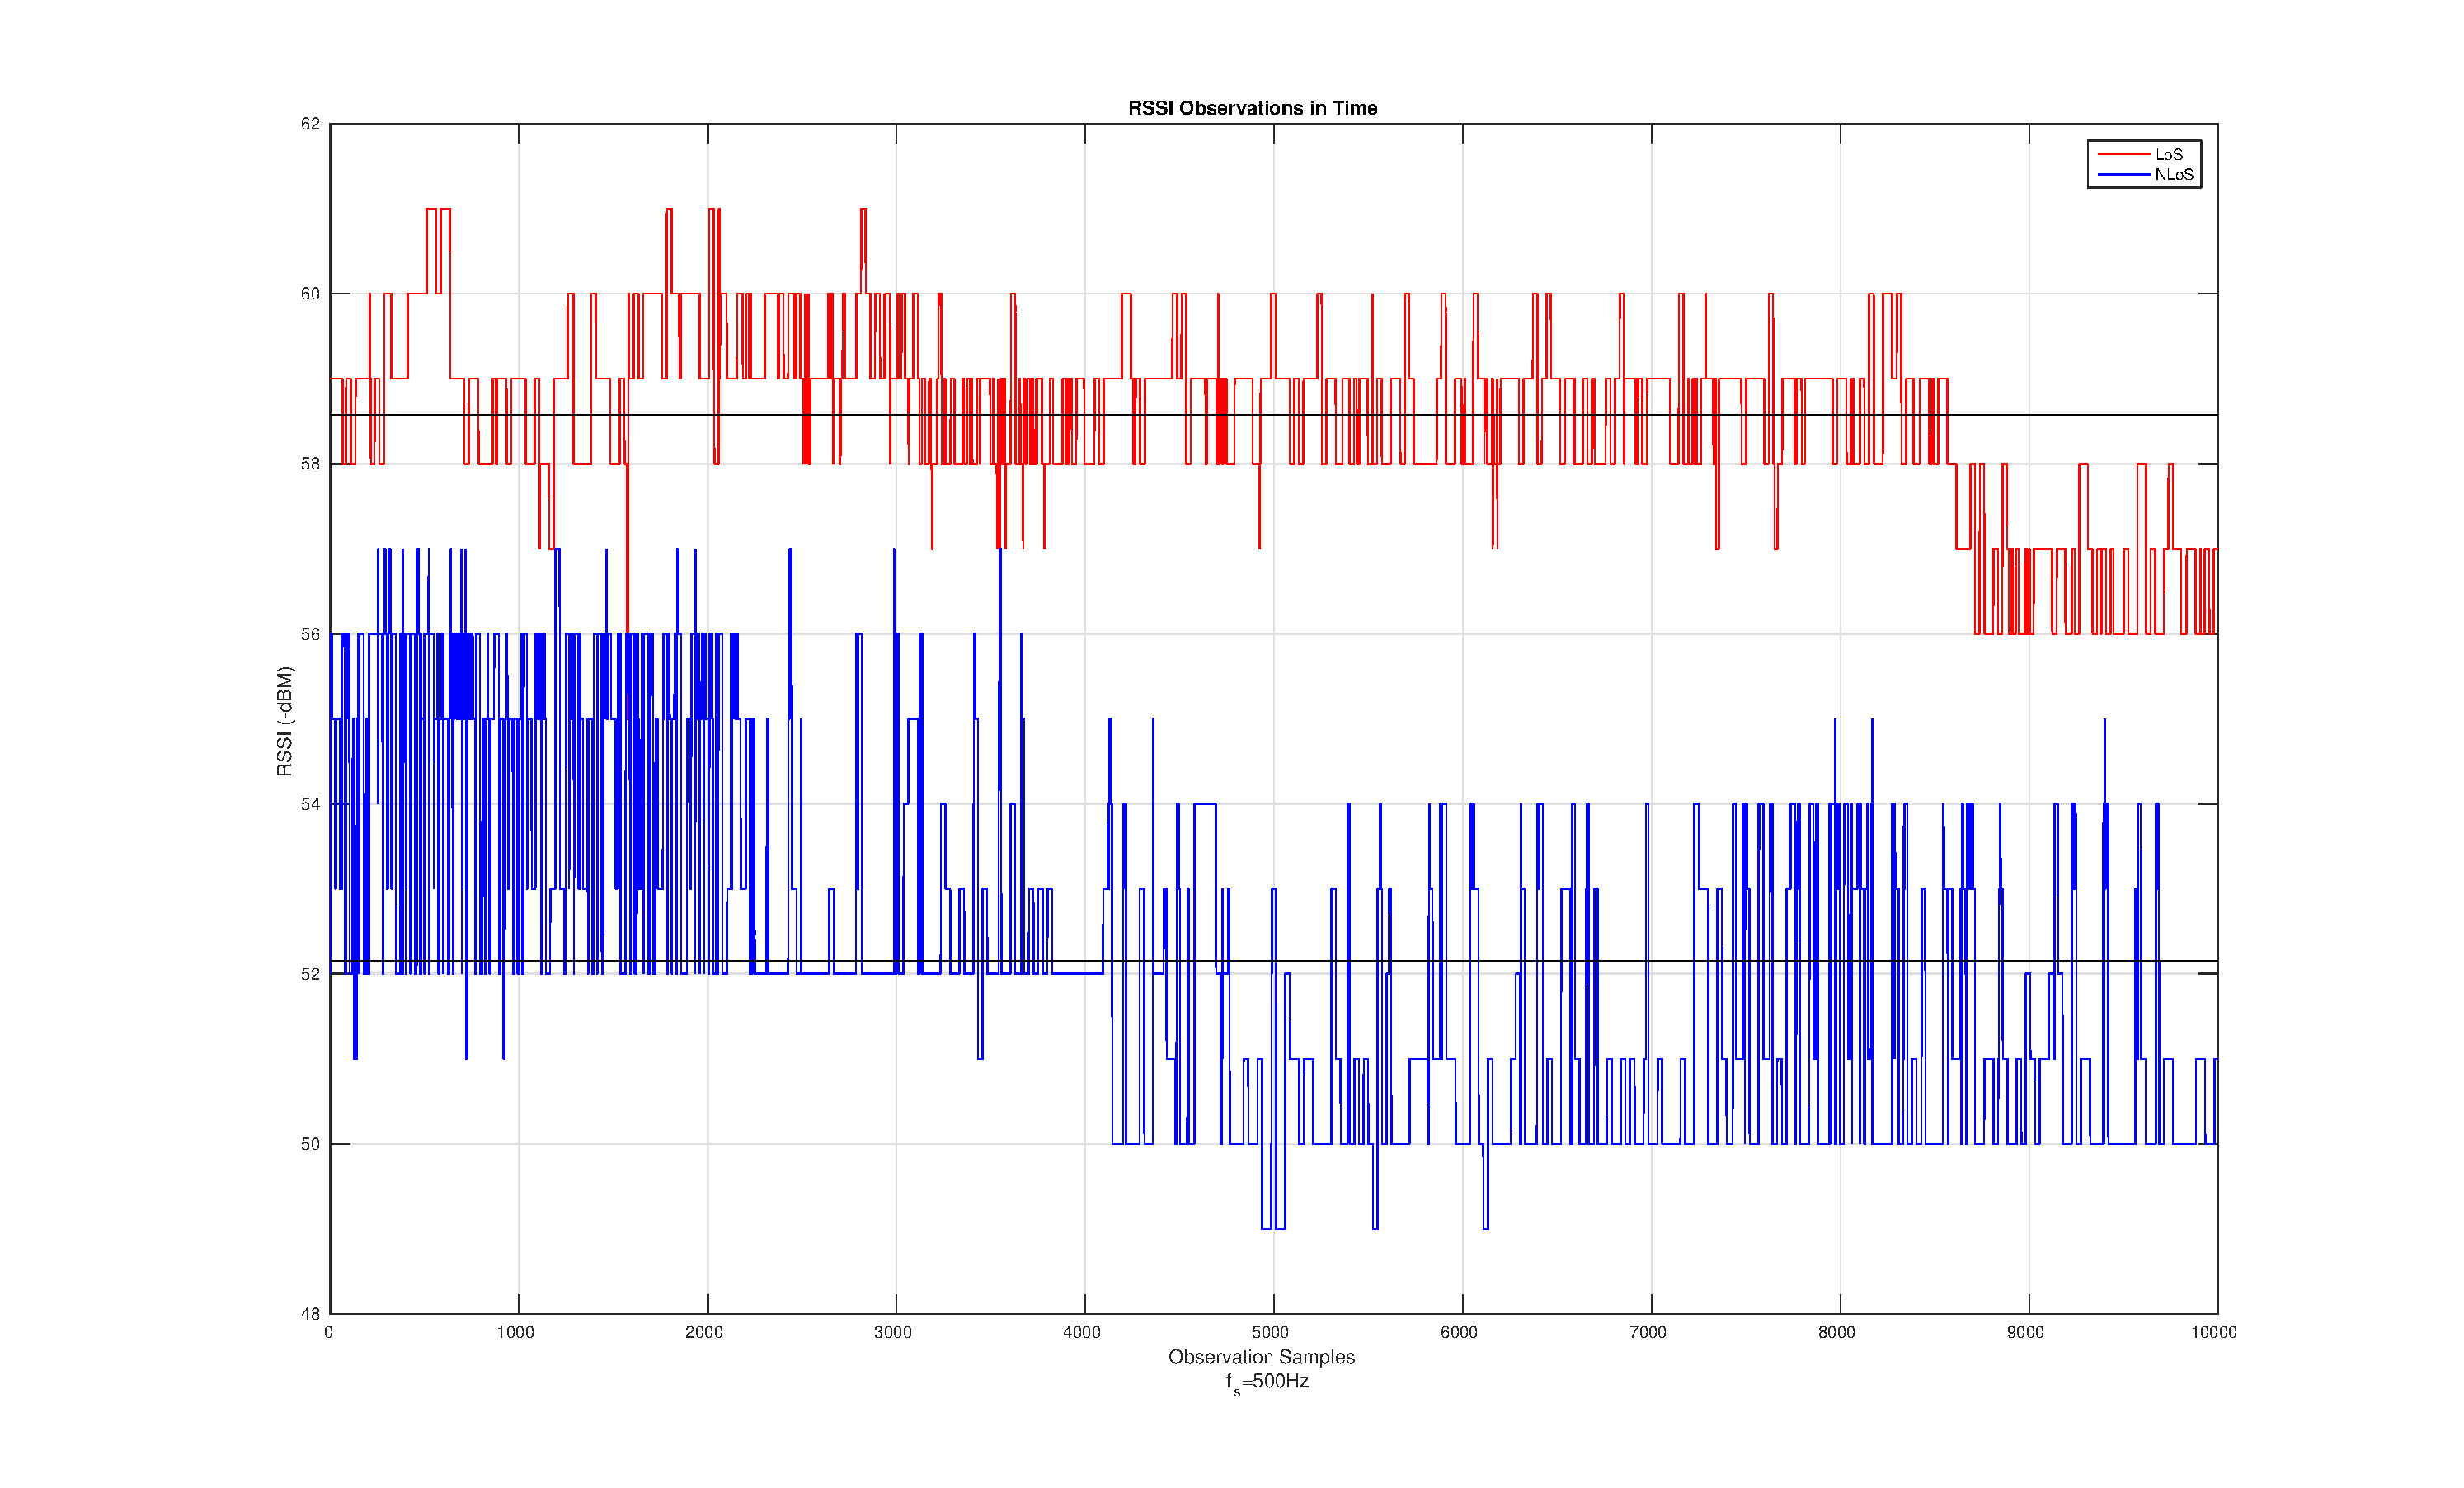
\includegraphics[scale=0.2]{figures/rssi_variance.eps}
       \caption{\label{fig-variance}RSSI readings of NLoS and LoS AP's acquired with a stationary agent}
    \end{figure}

    % \begin{itemize}
    %   \item CSI-related special \\
    %     hardware requirement
    %   \item Propagation-modelling \\
    %     multi-path effect difficult to model
    %   \item Fingerprinting \\
    %     An emerging area learning fingerprints is deep learning~\cite{gao2015channel}
    % \end{itemize}
